% In 2021 umgeschrieben, da sich kaum einer mehr ans Diplom erinnert. Fokus jetzt mehr auf Ba-Ma-System anstatt Historie.
\section{Das Bachelor-Master-System im Schnelldurchlauf}

\begin{multicols}{2}
\begin{quote}
	\textit{\foreignlanguage{english}{I accept chaos, I'm not sure whether it accepts me.}}

	\hfill--- Bob Dylan
\end{quote}
Bevor wir euch die einzelnen Physikstudiengänge im Detail vorstellen, soll es kurz um das zugrundeliegende System von Bachelor- und Masterabschlüssen gehen.
Diese gibt es mittlerweile zwar schon seit rund zwei Jahrzehnten und sie sind den meisten ein Begriff, ein kleiner Exkurs zur Geschichte ist dennoch sinnvoll.
Eingeführt wurde das Bachelor-Master-System in Deutschland im Zuge des Bologna-Prozess um die Jahrtausendwende und ersetzte damit das Diplomstudium.
Das stellte nicht nur eine große Veränderung für die Hochschulen dar, sondern gab auch diesem Artikel seine Grundlage.
Ging es zunächst noch darum, einen Leitfaden durch das anfängliche Chaos zu schreiben, mit nostalgischem Unterton über den Verlust des Diplomstudiums, so mussten wir den Text über die Jahre mehrfach anpassen. Heute hat sich das Bachelor-Master-System etabliert und nostalgische Rückblicke sind nur noch bei den wenigsten Professorinnen und Professoren zu finden.
Aber der Reihe nach: Die Bologna-Reform machte aus dem Grundstudium im Diplom den Bachelor und aus dem Hauptstudium den Master, mit der Idee die Studiengänge europaweit zu vereinheitlichen.

\textbf{Wichtige Ziele der Deklaration:}
\begin{itemize}
	\item die Schaffung eines Systems leicht verständlicher und vergleichbarer Abschlüsse
	\item Förderung der Mobilität (Erasmus, Erasmus+)
	\item Förderung der europäischen Zusammenarbeit im Bereich der Qualitätssicherung
\end{itemize}

Hierzu wurden Vorlesungen, Übungen etc. nun als Module mit abschließender Klausur und Endnote zusammengefasst, über die dann die erforderlichen Credits/Leistungspunkte gesammelt werden und durch die Zweistufigkeit sollte bereits der Bachelor als berufsqualifizierender Abschluss dienen.
In Deutschland hat es sich etabliert, den Bachelor auf 3~Jahre anzusetzen mit einem anschließenden zweijährigen Master.

So viel Veränderung hat die Hochschulen zunächst überfordert, zumal auch noch elektronische Prüfungssysteme wie das QISPOS eingeführt wurden. Mittlerweile ist das neue System aber gar nicht mehr so neu und verwirrend und es lässt sich bereits ein erstes Fazit ziehen:
Als besonders positiv hat sich die hohe Anrechenbarkeit von international absolvierten Credits gezeigt, was sich insbesondere in der Anzahl an absolvierten Auslandsaufenthalten zeigt. Zudem ist durch die Zweistufigkeit ein Wechsel nach dem Bachelor in einen anderen Master leicht möglich, insbesondere bei Physik lässt dies einen hohen Grad an Spezial-Mastern zu.
Es bleibt nur zu hoffen, dass hier auch in Zukunft genügend Masterplätze zur Verfügung stehen.
Als Kritikpunkt wird oft angeführt, dass durch die strikten Modulvorgaben die individuelle Entfaltung der Studierenden zu kurz kommt und auch der Bachelor als berufsqualifizierender Abschluss konnte sich in der Praxis nicht durchsetzen. Meistens ist der anschließende Masterabschluss notwendig.

Es bleibt zu hoffen, dass die Diskussion über die Reformen weiterlebt und auch dieser Artikel in Zukunft von weiteren Verbesserungen berichten kann.

\fibelsig{Connie, Simon, Moritz}
\end{multicols}

\begin{center}
	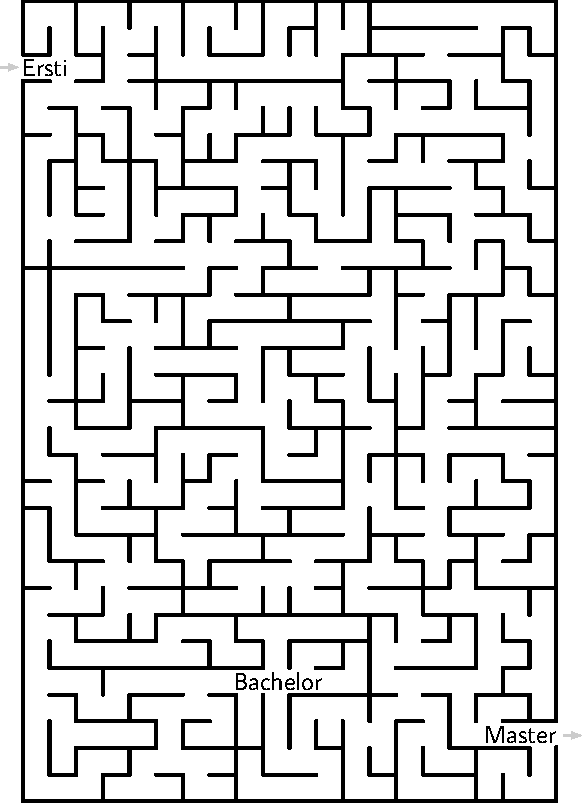
\includegraphics[width=\textwidth, height=0.38\textheight]{res/bachelor_master_labyrinth.pdf}
\end{center}
